\documentclass{standalone} % DO NOT CHANGE THIS
\usepackage{tikz}
\usepackage[utf8]{inputenc}
\usepackage{graphicx}
\usepackage{times}
\usepackage{amssymb}
\usetikzlibrary[arrows.meta, positioning,math, calc, shapes.geometric, intersections, fit, backgrounds, decorations.pathmorphing]

\begin{document}

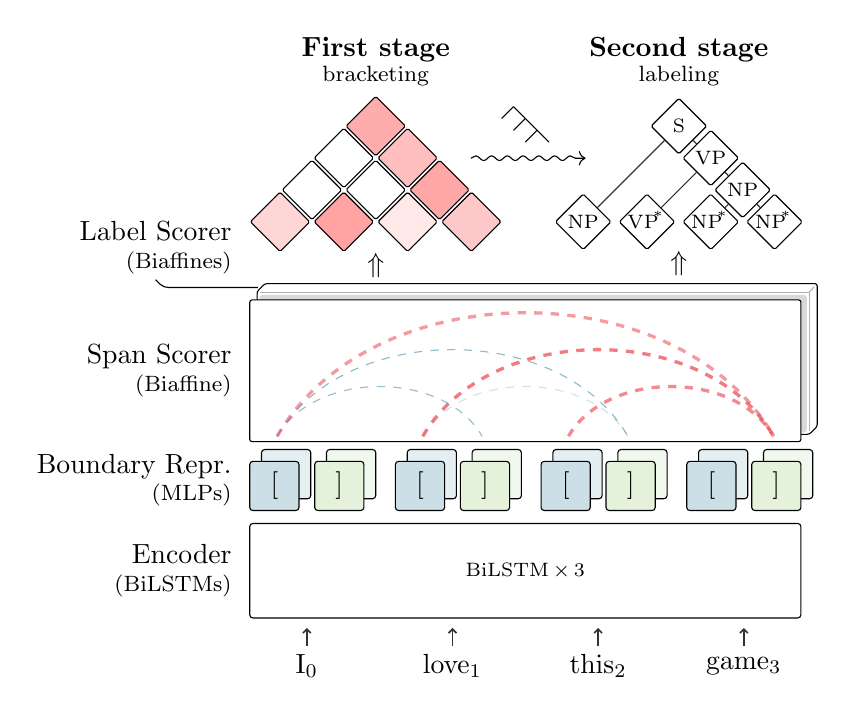
\begin{tikzpicture}[
    connect/.style={
            rounded corners=4pt,
            semithick,
            draw=black!80
        },
    arrow/.style={
            % >=latex,
            arrows = {-Straight Barb[length=0.5mm]},
            shorten >= 2pt,
            shorten <= 1.5pt,
            thin
        },
    inner arrow/.style={
            % arrows = {-Straight Barb[length=0.7mm]},
            dashed,
            shorten >= 2pt,
            shorten <= 2pt,
            thin,
            draw=black!50
        },
    input/.style={
            rectangle,
            %   thick,
            draw=none,
            % fill=white,
            minimum height=0.4cm,
            %   fill=orange!10,
            %   draw=orange!40
            %   fill={rgb,255:red,255; green,239; blue,213},
            %   draw={rgb,255:red,225; green,209; blue,183},
        },
    share/.style={
            minimum height=0.5cm,
            %   fill=orange!10,
            %   draw=orange!40,
            % fill={rgb,255:red,255; green,239; blue,213},
            %   fill,
            %   right color={rgb,255:red,204; green,223; blue,230},
            %   left color={rgb,255:red,228; green,242; blue,220},
            % draw={rgb,255:red,225; green,209; blue,183},
            draw=black,
            rounded corners=2mm,
        },
    task2/.style={
            minimum height=0.5cm,
            % fill=white,
            fill={rgb,255:red,228; green,242; blue,220},
            % draw={rgb,255:red,187; green,217; blue,186},
            draw=black,
            rounded corners=2mm,
        },
    label/.style={
            inner sep=0.5mm,
            fill=white,
            minimum height=0.5cm,
        },
    task1/.style={
            minimum height=0.5cm,
            % fill=black!30,
            fill={rgb,255:red,204; green,223; blue,230},
            % draw={rgb,255:red,151; green,181; blue,191},
            draw=black,
            rounded corners=2mm
        },
    inner lstm/.style={
            fill=white,
            rectangle,
            rounded corners=1mm,
            semithick,
            draw=black,
            fill opacity=0.8
        },
    cell/.style={
            inner sep=2mm,
            rectangle,
            rounded corners=1mm,
            semithick,
            draw=black,
        },
    chart/.style={
            diamond,
            minimum size=7.6mm,
            rounded corners=0.2mm,
            draw=black,
            % thin,
        },
    ocell/.style={
            solid,
            minimum height=0.5cm,
            rectangle,
            rounded corners=0.4mm,
        },
    dep arrow/.style={
    arrows = {-Latex[round,open,length=8pt,width=6pt]},
    shorten >= 2pt,
    shorten <= 1.5pt,
    thick
    },
    post score/.style={
            fill=red!50,
            draw={rgb,255:red,238; green,89; blue,100},
        },
    neg score/.style={
            draw={rgb,255:red,93; green,157; blue,177},
        },
    ]
    \centering

    %\scriptsize BiLSTM
    \node [share, ocell] [minimum width=7cm, minimum height=1.2cm, anchor=south] (lstm) {\scriptsize BiLSTM$\, \times \, 3$};

    \node [share, ocell, draw=none, fill=none] [minimum width=7cm, minimum height=1.8cm, anchor=south west] (label biaffine') at ($(lstm.north west) + (0.2, 1.225)$) {};

    \node [share, ocell, draw=none, fill=none] [minimum width=7cm, minimum height=1.8cm, anchor=south west] (label biaffine) at ($(lstm.north west) + (0.1, 1.125)$) {};

    \node [share, ocell, draw=none, fill=black!15] [minimum width=6.95cm, minimum height=1.75cm] at ($(label biaffine) + (0, -0.01)$) {};

    \draw [black, rounded corners=0.3mm] (label biaffine.south west) -- (label biaffine.south east) -- (label biaffine'.south east) -- (label biaffine'.north east) -- (label biaffine'.north west) -- (label biaffine.north west) -- cycle;

    \draw [black!30] ($(label biaffine.north west) + (0.04, -0.01)$) -- ($(label biaffine.north east) + (0, -0.01)$) -- ($(label biaffine.south east) + (0, +0.04)$);

    \draw [black!30] ($(label biaffine.north east) + (0, -0.01)$) -- ($(label biaffine'.north east) + (-0.04, -0.04)$);

    \node [draw=black, fill=white, rounded corners=0.3mm] [minimum width=7cm, minimum height=1.8cm, anchor=south west] (biaffine) at ($(lstm.north west) + (0, 1.025)$) {};

    \node [task1, ocell, minimum size=0.625cm, anchor=south west] (f0) at ($(lstm.north west) + (0, 0.15)$) {[};
    \node [task2, ocell, minimum size=0.625cm, anchor=south west] (b0) at ($(lstm.north west) + (0.825, 0.15)$) {]};

    \node [task1, ocell, minimum size=0.625cm, anchor=south west] (f1) at ($(lstm.north west) + (1.85, 0) + (0, 0.15)$) {[};
    \node [task2, ocell, minimum size=0.625cm, anchor=south west] (b1) at ($(lstm.north west) + (1.85, 0) + (0.825, 0.15)$) {]};

    \node [task1, ocell, minimum size=0.625cm, anchor=south west] (f2) at ($(lstm.north west) + (3.7, 0) + (0, 0.15)$) {[};
    \node [task2, ocell, minimum size=0.625cm, anchor=south west] (b2) at ($(lstm.north west) + (3.7, 0) + (0.825, 0.15)$) {]};

    \node [task1, ocell, minimum size=0.625cm, anchor=south west] (f3) at ($(lstm.north west) + (5.55, 0) + (0, 0.15)$) {[};
    \node [task2, ocell, minimum size=0.625cm, anchor=south west] (b3) at ($(lstm.north west) + (5.55, 0) + (0.825, 0.15)$) {]};

    \begin{scope}[on background layer]
        \node [task1, ocell, minimum size=0.625cm, anchor=south west, fill opacity=0.5] (f0') at ($(lstm.north west) + (0.15, 0.3)$) {};
        \node [task2, ocell, minimum size=0.625cm, anchor=south west, fill opacity=0.5] (b0') at ($(lstm.north west) + (0.975, 0.3)$) {};

        \node [task1, ocell, minimum size=0.625cm, anchor=south west, fill opacity=0.5] (f1') at ($(lstm.north west) + (1.85, 0) + (0.15, 0.3)$) {};
        \node [task2, ocell, minimum size=0.625cm, anchor=south west, fill opacity=0.5] (b1') at ($(lstm.north west) + (1.85, 0) + (0.975, 0.3)$) {};

        \node [task1, ocell, minimum size=0.625cm, anchor=south west, fill opacity=0.5] (f2') at ($(lstm.north west) + (3.7, 0) + (0.15, 0.3)$) {};
        \node [task2, ocell, minimum size=0.625cm, anchor=south west, fill opacity=0.5] (b2') at ($(lstm.north west) + (3.7, 0) + (0.975, 0.3)$) {};

        \node [task1, ocell, minimum size=0.625cm, anchor=south west, fill opacity=0.5] (f3') at ($(lstm.north west) + (5.55, 0) + (0.15, 0.3)$) {};
        \node [task2, ocell, minimum size=0.625cm, anchor=south west, fill opacity=0.5] (b3') at ($(lstm.north west) + (5.55, 0) + (0.975, 0.3)$) {};
    \end{scope}

    \draw [inner arrow, connect, neg score, fill=none, thin, draw opacity=0.65] [out=60,in=120,looseness=1] ($(f0.north) + (0, 0.25)$) to ($(b1.north) + (0, 0.25)$);
    \draw [inner arrow, connect, neg score, fill=none, thin, draw opacity=0.7] [out=60,in=120,looseness=1] ($(f0.north) + (0, 0.25)$) to ($(b2.north) + (0, 0.25)$);
    \draw [inner arrow, connect, post score, fill=none, very thick, draw opacity=0.6] [out=60,in=120,looseness=1] ($(f0.north) + (0, 0.25)$) to ($(b3.north) + (0, 0.25)$);

    \draw [inner arrow, connect, neg score, fill=none, thin, draw opacity=0.30] [out=60,in=120,looseness=1] ($(f1.north) + (0, 0.25)$) to ($(b2.north) + (0, 0.25)$);
    \draw [inner arrow, connect, post score, fill=none, very thick, draw opacity=0.8] [out=60,in=120,looseness=1] ($(f1.north) + (0, 0.25)$) to ($(b3.north) + (0, 0.25)$);

    \draw [inner arrow, connect, post score, fill=none, very thick, draw opacity=0.7] [out=60,in=120,looseness=1] ($(f2.north) + (0, 0.25)$) to ($(b3.north) + (0, 0.25)$);

    \node (p0) at ($(f0.south)!0.5!(b0.south)$) {};
    \node (p1) at ($(f1.south)!0.5!(b1.south)$) {};
    \node (p2) at ($(f2.south)!0.5!(b2.south)$) {};
    \node (p3) at ($(f3.south)!0.5!(b3.south)$) {};

    \node [input, inner sep=0pt, anchor=north] (input0) at ($(lstm.south -| p0) - (0, 0.4cm)$) {I$_0$};

    \node [input, inner sep=0pt, anchor=north] (input1) at ($(lstm.south -| p1) - (0, 0.4cm)$) {love$_1$};

    \node [input, inner sep=0pt, anchor=north] (input2) at ($(lstm.south -| p2) - (0, 0.4cm)$) {this$_2$};

    \node [input, inner sep=0pt, anchor=north] (input3) at ($(lstm.south -| p3) - (0, 0.4cm)$) {game$_3$};


    \draw [arrow, connect] (input0) -- ($(lstm.south -| input0) - (0, 0.05cm)$);
    \draw [arrow, connect] (input1) -- ($(lstm.south -| input1) - (0, 0.05cm)$);
    \draw [arrow, connect] (input2) -- ($(lstm.south -| input2) - (0, 0.05cm)$);
    \draw [arrow, connect] (input3) -- ($(lstm.south -| input3) - (0, 0.05cm)$);

    \node [post score, chart, fill opacity=0.65] (chart_c) at ($(biaffine.north) + (-1.9cm, 2.2cm)$) {};

    \node [neg score, chart, fill opacity=0.7] at ($(chart_c) + (-0.405, -0.405)$) {};
    \node [post score, chart, fill opacity=0.5] at ($(chart_c) + (0.405, -0.405)$) {};

    \node [neg score, chart, fill opacity=0.8] at ($(chart_c) + (-0.81, -0.81)$) {};
    \node [neg score, chart, fill opacity=0.3] at ($(chart_c) + (0, -0.81)$) {};
    \node [post score, chart, fill opacity=0.7] at ($(chart_c) + (0.81, -0.81)$) {};

    \node [post score, chart, fill opacity=0.324] (chart_b0) at ($(chart_c) + (-1.215, -1.215)$) {};
    \node [post score, chart, fill opacity=0.723] at ($(chart_c) + (-0.405, -1.215)$) {};
    \node [post score, chart, fill opacity=0.173] at ($(chart_c) + (0.405, -1.215)$) {};
    \node [post score, chart, fill opacity=0.432] (chart_b3) at ($(chart_c) + (1.215, -1.215)$) {};

    \node (placeholder_chart) [inner sep=0mm, fit=(chart_c) (chart_b0) (chart_b3)] {};


    \node [draw=black!50, chart, minimum size=7.1mm] (chart_c') at ($(biaffine.north) + (1.95cm, 2.2cm)$) {};


    \node [draw=black!50, chart, minimum size=7.1mm] (chart_11') at ($(chart_c') + (0.405, -0.405)$) {};


    \node [draw=black!50, chart, minimum size=7.1mm] (chart_21') at ($(chart_c') + (0.81, -0.81)$) {};


    \node [draw=black!50, chart, minimum size=7.1mm] (chart_b0') at ($(chart_c') + (-1.215, -1.215)$) {};
    \node [draw=black!50, chart, minimum size=7.1mm] (chart_31') at ($(chart_c') + (-0.405, -1.215)$) {};
    \node [draw=black!50, chart, minimum size=7.1mm] (chart_32') at ($(chart_c') + (0.405, -1.215)$) {};
    \node [draw=black!50, chart, minimum size=7.1mm] (chart_b3') at ($(chart_c') + (1.215, -1.215)$) {};

    \begin{scope}
        \node [anchor=base] at ($(chart_c') + (0, -0.085cm)$) {\scriptsize{S}};
        \node [anchor=base] at ($(chart_11') + (0, -0.085cm)$) {\scriptsize{VP}};
        \node [anchor=base] at ($(chart_21') + (0, -0.085cm)$) {\scriptsize{NP}};
        \node [anchor=base] at ($(chart_b0') + (0, -0.085cm)$) {\scriptsize{NP}};
        \node [anchor=base] at ($(chart_31') + (-0.05, -0.085cm)$) {\scriptsize{VP}};
        \node [anchor=base] at ($(chart_32') + (-0.05, -0.085cm)$) {\scriptsize{NP}};
        \node [anchor=base] at ($(chart_b3') + (-0.05, -0.085cm)$) {\scriptsize{NP}};
        \node [anchor=base] at ($(chart_31') + (0.14, 0.06)$) {\tiny{$\ast$}};
        \node [anchor=base] at ($(chart_32') + (0.14, 0.06)$) {\tiny{$\ast$}};
        \node [anchor=base] at ($(chart_b3') + (0.14, 0.06)$) {\tiny{$\ast$}};
    \end{scope}

    \node (placeholder_chart') [inner sep=0mm, fit=(chart_c') (chart_b0') (chart_b3')] {};

    \draw [draw=black!80] (chart_c') -- (chart_b0');
    \draw [draw=black!80] (chart_c') -- (chart_11');
    \draw [draw=black!80] (chart_11') -- (chart_31');
    \draw [draw=black!80] (chart_11') -- (chart_21');
    \draw [draw=black!80] (chart_21') -- (chart_32');
    \draw [draw=black!80] (chart_21') -- (chart_b3');

    \draw [->, decorate, decoration={snake,amplitude=.3mm,segment length=2mm,post length=1mm}] ($(placeholder_chart.east) + (-0.4, 0.2)$) -- ($(placeholder_chart'.west) + (0.4, 0.2)$);

    \begin{scope}[
            level distance=1.5mm,
            yshift=6.5cm,
            xshift=-1.5mm,
            level/.style={sibling distance=3mm},
            % xshift=-1mm,
            % level 1/.style={sibling distance=3mm},
            % level 2/.style={sibling distance=2mm},
            % level 3/.style={sibling distance=1mm}
        ]
        \coordinate
        child
        child {child child {child child}};
    \end{scope}

    \node at ($(label biaffine'.north -| placeholder_chart)!0.6!(placeholder_chart.south)$) {$\Uparrow$};

    \node at ($(label biaffine'.north -| placeholder_chart')!0.6!(placeholder_chart'.south)$) {$\Uparrow$};

    \node [anchor=east, align=right] at ($(lstm.west) + (-0.1, 0)$) {Encoder\\[-2pt]\footnotesize (BiLSTMs)};

    \node [anchor=east, align=right] at ($(f0.west) + (-0.1, 0.075)$) {Boundary Repr.\\[-2pt]\footnotesize (MLPs)};

    \node [anchor=east, align=right] (biaffine) at ($(biaffine.west) + (-0.1, 0)$) {Span Scorer\\[-2pt]\footnotesize (Biaffine)};

    \node [anchor=south east, align=right] (biaffine label) at ($(label biaffine.north west) + (-0.2, +0.1)$) {Label Scorer\\[-2pt]\footnotesize (Biaffines)};

    \draw [rounded corners=0.6mm] ($(biaffine label.south) + (0, 0.05)$)-- ($(biaffine label.south) + (0.1, -0.05)$) -- ($(biaffine label.south east) + (0.21, -0.05)$);

    % \node [anchor=east] at ($(biaffine label.east |- placeholder_chart)$) {\scriptsize Inside/CKY (CRF)};

    \node [anchor=south, align=center] at ($(placeholder_chart.north)$) {\textbf{First stage}\\[-3pt]\footnotesize bracketing};

    \node [anchor=south, align=center] at ($(placeholder_chart'.north) + (0, 0.25mm)$) {\textbf{Second stage}\\[-3pt]\footnotesize labeling};

\end{tikzpicture}
\end{document}

